\documentclass[border=6pt,tikz]{standalone}
\usepackage{tikz}
\usepackage{amsmath,amssymb}
\usetikzlibrary{arrows.meta,positioning,fit,backgrounds,calc,shapes.geometric,decorations.pathreplacing,patterns}
\definecolor{ink}{HTML}{1B2430}
\definecolor{muted}{HTML}{6B7785}
\definecolor{accent}{HTML}{2F6FB5}
\definecolor{accent2}{HTML}{C1611F}
\definecolor{good}{HTML}{2E7D5B}
\definecolor{soft}{HTML}{EDF2F7}
\definecolor{soft2}{HTML}{FBEDE2}
\definecolor{soft3}{HTML}{E6F0E9}
\tikzset{
  box/.style={draw=ink,line width=.7pt,rounded corners=2pt,fill=soft,inner sep=4pt,align=center,font=\sffamily\small},
  boxa/.style={box,fill=soft2},
  boxb/.style={box,fill=soft3},
  plain/.style={align=center,font=\sffamily\small,text=ink},
  tiny/.style={align=center,font=\sffamily\scriptsize,text=muted},
  ar/.style={-{Stealth[length=2.4mm]},draw=ink,line width=.7pt},
  arm/.style={-{Stealth[length=2.4mm]},draw=muted,line width=.6pt,dashed},
  nd/.style={circle,draw=ink,line width=.7pt,fill=white,minimum size=7mm,inner sep=0pt,font=\sffamily\scriptsize},
  ndf/.style={nd,fill=soft},
  ndt/.style={nd,fill=soft2},
}

\begin{document}

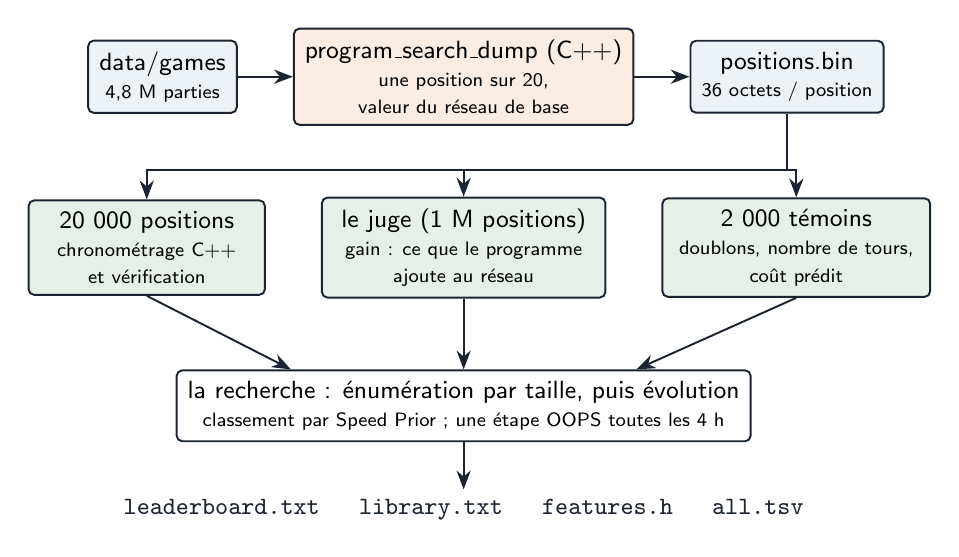
\begin{tikzpicture}[node distance=4mm and 7mm]
\node[box] (games) {data/games\\[-1pt]\scriptsize 4,8 M parties};
\node[boxa,right=of games] (dump) {program\_search\_dump (C++)\\[-1pt]\scriptsize une position sur 20,\\[-1pt]\scriptsize valeur du réseau de base};
\node[box,right=of dump] (pos) {positions.bin\\[-1pt]\scriptsize 36 octets / position};
\node[boxb,below=9mm of dump,minimum width=36mm] (scorer) {le juge (1 M positions)\\[-1pt]\scriptsize gain : ce que le programme\\[-1pt]\scriptsize ajoute au réseau};
\node[boxb,right=of scorer,minimum width=34mm] (wit) {2 000 témoins\\[-1pt]\scriptsize doublons, nombre de tours,\\[-1pt]\scriptsize coût prédit};
\node[boxb,left=of scorer,minimum width=30mm] (harn) {20 000 positions\\[-1pt]\scriptsize chronométrage C++\\[-1pt]\scriptsize et vérification};
\node[box,below=9mm of scorer,minimum width=64mm,fill=white] (search) {la recherche : énumération par taille, puis évolution\\[-1pt]\scriptsize classement par Speed Prior ; une étape OOPS toutes les 4 h};
\node[plain,below=6mm of search] (out) {\ttfamily leaderboard.txt \quad library.txt \quad features.h \quad all.tsv};
\draw[ar] (games) -- (dump);
\draw[ar] (dump) -- (pos);
\draw[ar] (pos.south) |- ($(wit.north)+(0,0.35)$) -| (wit.north);
\draw[ar] (pos.south) |- ($(wit.north)+(0,0.35)$) -| (scorer.north);
\draw[ar] (pos.south) |- ($(wit.north)+(0,0.35)$) -| (harn.north);
\draw[ar] (scorer) -- (search);
\draw[ar] (wit.south) -- ($(search.north east)!0.2!(search.north west)$);
\draw[ar] (harn.south) -- ($(search.north west)!0.2!(search.north east)$);
\draw[ar] (search) -- (out);
\end{tikzpicture}
\end{document}
